\subsection{Data Plane Strategies}

\begin{task}
\label{task:system:dataplane}
We will design and implement efficient data-plane implementations to
guarantee \blue{reachability and consistency properties}, in presence
of reconfiguration and link dynamics.
\end{task}

\smallskip

In translating the JRTE solution into a consistent and efficient data
plane forwarding strategy, we build upon recent advances in
software-defined networking (SDN), as it provides cleaner management
abstractions and open interfaces (e.g., via APIs such as
OpenFlow~\cite{}). However, \ArchName introduces unique challenges.
In particular, in face of a dynamically changing network due to
reconfigurations, we need to ensure that: (a) packets do not use
deactivated links \blue{(i.e., black holes~\cite{} are avoided)}, (b)
the network remains connected at all times, and (c) the packet latency
remains bounded. Finally, we also need a data plane strategy to: (d)
handle transient misalignment of FSO links. We note that the recent
related works either assume a {\em static}
network~\cite{cons-update,incconsupdate} or focus on a single
reconfiguration~\cite{cu-1}, and hence, are not directly applicable to
our context.

\para{\underline{(a) and (b).} Avoiding Black Holes, and Guaranteeing
  Connectivity.}  Packets are routed in the network on the basis of
forwarding tables, which essentially specify, at each node, the next
hop/link to use for each destination. In a dynamic network, forwarding
tables will also be changing constantly.  Note that
activation/deactivation of a link \blue{may take a few tens of msecs,
  and that we cannot directly update the tables across all the network
  switches in one atomic action.}
%
In face of these challenges, we need to ensure that through every
possible intermediate state of the switches' tables and links, the
forwarding tables always refer to only active links. We can ensure
this by a careful ordering of steps as suggested in our preliminary
work~\cite{hotnets}. In particular, (i) we reflect removal of links in
the forwarding tables, before actually deactivating the links, and
(ii) reflect addition of links in the tables only after the link
activation is complete. The above solution works irrespective of the
order in which the forwarding tables are updated across the network,
and even in the presence of multiple concurrent reconfigurations. 

In addition to above, we also need to ensure that the network remains
connected at all times. There are two possible solutions to this: (i)
maintain a static ``backbone'' subnetwork that ensures connectivity,
or (ii) reject reconfigurations that disconnect the network. The first
approach reduces the degree of flexibility in network design and
\blue{could result in poor performance.} The second approach requires
a careful implementation if there are multiple {\em concurrent}
reconfigurations. Concurrent reconfigurations can be handled in three
ways: (i) one at a time, (ii) in batches (i.e., queue and combine them
into a single reconfiguration); and (iii) execute each reconfiguration
individually but {\em concurrently}. The first two options introduce
unnecessary reconfiguration delays, while the third option requires a
careful implementation to ensure correctness---we need to keep a
single consistent view of the network topology graph and allow only
{\em atomic} access to it (when checking if a reconfiguration
disconnents the network). \eat{Again, the above solutions work
  irrespecitve of the order in which the forwarding tables are updated
  across the network.} In our research, we will study and compare the
performance of such approaches.

\begin{wrapfigure}{r}{0.3\textwidth}
\vspace{-0.4cm}
\centering
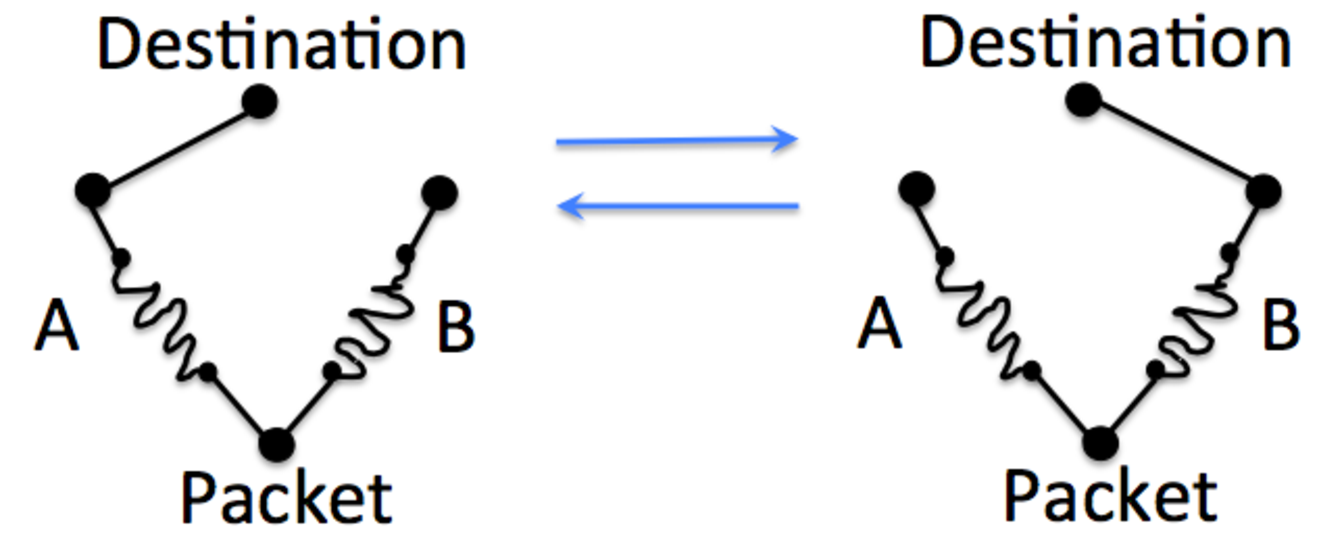
\includegraphics[width=150pt]{PPTFigs/impossible.pdf}
\caption{If the network goes back and forth between the above
  topologies (due to corresponding reconfigurations), then the packet
  will continue to ``swing'' between areas A and B---leading to a
  (perennial) forwarding ``loop''.}
\label{fig:impossible}
\end{wrapfigure}
\para{\underline{(c)} Guaranteeing Bounded Packet Latency.}  The above
strategies still do not guarantee a bounded packet latency. In fact,
in general, its {\em impossible} to guarantee bounded packet latency
(e.g., see Figure~\ref{fig:impossible}). 
%
However, such situations can be avoided if we ensure a minimum time
interval between consecutive reconfigurations; this minimum interval
is also essential for the centralized controlled and the wireless
control channel to be able to handle the resulting load (see
Section~\ref{sec:wireless}.)  In particular, we can formally prove
that a minimum interval of $(x + y)$ time units between
reconfigurations suffices to ensure an upper bound of $2x$ units on
packet latency, where $x$ is the bound on packet latency given a fixed
network and $y$ is the maximum time taken to update (not necessarily
atomically) the network forwarding tables.
%
We can expect $x$ and $y$ to be of the order of 1-2 msecs. Note that
the above claim is independent of the link activation or deactivation
latency (which can be a few tens of msecs).

\para{\underline{(d)} Handling Misalignment of Links.} In \ArchName,
even during a static topology state, links may be temporarily
unavailable because of possible misalignment of the FSO
links. \blue{Such misalignments are fixed in real-time by mechanisms
  suggested in Section~\ref{sec:fso}} in timescales much smaller than
the time needed to update rules~\cite{ddcnsdi13} by an SDN
controller. In fact, it may even be counterproductive to report such
transient link failures to the controller, as it may cause needless
update of forwarding tables. Thus, we need appropriate \blue{network
  layer} techniques to recover from such transient link
failures. \blue{Future SDN roadmaps have provisions for local recovery
  mechanisms analogous to similar schemes in the MPLS and SONET
  literature~\cite{}. We will explore the available alternatives in
  our research. In the absence of such features,} we will investigate
design of a local ``lightweight'' SDN controller on every rack that
can quickly react to such misalignments.
